% ============================================================================
% Nature Machine Intelligence submission
% Paper 0 (NSF AI Agent Project) --- reframed from the AAAI-style "Behavioral
% Ceiling" manuscript at paper0_ai_agent_theory/latex/main.tex. The AAAI
% version is preserved as backup; this file reframes the same empirical
% content around a single, broadly interdisciplinary claim: that purely
% behavioral detection of AI agents in digital markets hits an
% information-theoretic ceiling that is within ~2 percentage points of what
% real classifiers already achieve.
% ============================================================================
\documentclass[11pt,a4paper]{article}

\usepackage[margin=1in]{geometry}
\usepackage{booktabs}
\usepackage{graphicx}
\usepackage{amsmath,amssymb,amsthm}
\usepackage{xcolor}
\usepackage{textcomp}
\usepackage{authblk}
\usepackage[hidelinks]{hyperref}
\usepackage{setspace}
\onehalfspacing

\title{Fundamental Information-Theoretic Limits of Behavioral\\ AI Agent Detection in Digital Markets}

\author[1]{NSF Project Team}
\affil[1]{Author affiliations withheld for double-blind review}

\date{}

\begin{document}
\maketitle

% ---------------------------------------------------------------------------
% ABSTRACT (target: 200 words)
% ---------------------------------------------------------------------------
\begin{abstract}
\noindent
Autonomous software agents now participate in digital markets, elections, and
public discourse, prompting regulators on three continents to draft
behavioral-detection regimes. We ask whether such regimes can, in principle,
identify AI agents from observable behavior alone. Using Fano's inequality,
we prove that any classifier that maps behavioral features $X$ to agent
category $Y$ obeys an accuracy ceiling determined by the mutual information
$I(X;Y)$ and the label entropy $H(Y)$. Applied to an 8-category taxonomy
spanning 2{,}744 blockchain addresses---a setting chosen because its public
transaction record allows exact measurement of $I(X;Y)$---we find a ceiling
of $97.2\%$; the best supervised classifier reaches $95.3\%$. The gap is
$1.7$--$4.6$ percentage points across feature sets: behavioral detection
is already near the information-theoretic limit. Unsupervised discovery saturates at
$2$--$3$ clusters regardless of feature set (HDBSCAN: $2$; K-Means silhouette:
$3$). A mechanistic decomposition separates two signal channels: execution
speed is a \emph{tool} signature (LLM-driven DeFi operations: median
$216$\,s vs.\ ${\sim}289$\,s for rule-based agents; Cohen's $d \approx 0$,
not a reliable difference) while inter-decision interval is an
\emph{agent} signature (general reaction time: $441$\,s vs.\ ${\sim}321$\,s;
Cohen's $d=1.01$). These findings imply that, on the Ethereum channel
studied, purely behavioral regulation faces a hard ceiling on
distinguishing agent categories; durable governance likely
requires either provenance registration or execution-layer signatures.
\end{abstract}

\vspace{0.5em}
\noindent\textbf{Keywords:} artificial intelligence; agent detection;
information theory; Fano's inequality; AI governance; digital markets.

% ===========================================================================
\section*{Introduction}
% ===========================================================================

Autonomous software agents---programs that perceive a digital environment,
decide without per-action human approval, and execute actions that move
money, vote, or speak---have left the laboratory. They trade on derivatives
venues, respond to constituents on social platforms, and settle governance
outcomes in distributed ledgers. Market analysts estimate that tens of
billions of U.S.\ dollars in annual transaction value on public blockchains
alone now flow through such agents\cite{daian2020flashboys,qin2022quantifying};
comparable (though harder to audit) activity occurs on advertising,
e-commerce and social platforms. The European Union's AI
Act\cite{eu_ai_act_2024}, the United States' Executive Order on AI
safety\cite{us_eo_14110}, and the United Kingdom's pro-innovation AI
regulation White Paper\cite{uk_ai_regulation_2023} all require that
``high-risk'' deployments be identified, disclosed, or certified. Each
proposal presupposes that AI agents can be reliably distinguished from
humans, from simple automation, and from one another.

The natural detection substrate is \emph{behavior}: an agent is known by its
actions in a public channel. Platforms that mandate real-name provenance
(such as certified identity registries) are legally and technically fragile
in the presence of pseudonymous participation, off-shore hosting, and
cross-border deployment. Behavior, by contrast, is visible everywhere a
platform offers an API. Almost every recent detection proposal---whether for
social-media bots\cite{varol2017,cresci2020detecting},
frontrunning agents\cite{daian2020flashboys,torres2021frontrunner}, coordinated
inauthentic behavior\cite{francois2020actors}, or
AI-generated content\cite{mitchell2023detectgpt,sadasivan2023}---therefore
relies on statistical classifiers trained on behavioral features. The
unstated assumption is that classifier accuracy can, in principle, be driven
arbitrarily close to 100\% by collecting more features, labeled data, or
model capacity.

The stakes of this assumption are not abstract. The rapid proliferation of
agentic foundation-model systems\cite{wang2024survey,xi2023rise,park2023generative,chan2023harms}
has focused policy-maker attention on three empirical questions. First,
\emph{how many} AI agents are now active in a given platform---a prevalence
question. Second, \emph{which kind} of AI agent is active at a given moment
of activity---a categorical question that underlies any
category-specific disclosure or risk assessment. Third, \emph{when} an
agent is acting on behalf of a human versus pursuing emergent objectives---a
question that underlies any accountability attribution. Every one of these
questions is typically answered, in practice, by training a behavioral
classifier; and every one is governed by the same information-theoretic
ceiling. Our analysis applies most directly to the categorical question,
but the methodology---estimate $I(X;Y)$, invert Fano, report the
head-room---generalizes to the others.

We show that this assumption is wrong, and quantify how wrong it is. Treating
the classification pipeline $X \to \hat{Y}$ as a communication channel,
Fano's inequality\cite{cover2006} supplies an accuracy ceiling that depends
only on the label entropy $H(Y)$ and the mutual information $I(X;Y)$ between
features and labels. We estimate both quantities directly on a corpus of
$2{,}744$ real agent deployments, using a setting in which the complete
action history is publicly observable: transactions on the Ethereum public
ledger. On this corpus, across three increasingly expressive behavioral
feature sets ($X_{23}$, $X_{31}$, $X_{47}$), the tightest achievable ceiling
is $97.2\%$. Real classifiers trained on the same data reach
$95.3\%$. \emph{The gap is roughly two percentage
points: behavioral detection is already at the information-theoretic limit.}

Crucially, this limit is not a consequence of dataset size, labeling noise,
or specific model choice. It is a property of the observation channel itself.
Adding features increases $I(X;Y)$ only up to a saturation point set by the
confusability of behavioral categories; beyond that point, further
engineering yields vanishing returns. We show this empirically: going from
$23$ to $47$ features raises the ceiling by less than one percentage point.

Three findings follow. First, a \emph{mechanistic} decomposition shows that
the residual signal lives almost entirely in inter-decision \emph{timing},
not in transactional content. LLM-driven agents show a nominally lower median DeFi execution time
than rule-based managers ($216$\,s vs.\ ${\sim}289$\,s), but this difference
is not statistically reliable (Cohen's $d \approx 0$, $p = 0.29$),
consistent with the tool-side code path being identical. Their general
inter-transaction interval, however, is reliably \emph{slower}
($441$\,s vs.\ ${\sim}321$\,s; $d = 1.01$), reflecting language-model
inference latency. Execution speed is thus a \emph{tool} signature
(indistinguishable across agent types); decision interval is an
\emph{agent} signature. Second, unsupervised discovery collapses: both
K-Means and density-based clustering (HDBSCAN) saturate at $2$--$3$ natural
behavioral clusters regardless of feature-set richness, even as the
taxonomy itself distinguishes eight. Third, the ceiling is \emph{channel-specific}: a replication on the
Polygon proof-of-stake chain, with different gas economics, yields a
cross-chain transfer accuracy of only $22.2\%$, demonstrating that
features calibrated on one chain do not transfer to another and that
each observation channel requires independent estimation of $I(X;Y)$.

The policy consequence is immediate. Behavioral regulation of AI agents is
structurally limited to coarse tiers (roughly: static automation,
rule-driven automation, adaptive agents). Finer-grained requirements---for
instance, stricter disclosure obligations specifically on LLM-driven
agents---\emph{cannot} be robustly enforced through behavioral observation.
Jurisdictions that require such distinctions will have to either (a)
mandate provenance registration at the point of deployment, or (b) compel
disclosure of execution-layer signatures (for example, cryptographic
attestations of the inference runtime). Our results give the first
principled, quantitative basis for this trade-off.

The choice of blockchain as a measurement substrate deserves brief
justification. The argument is domain-general, but the quantitative claim
requires that we \emph{know} the ground-truth categories for a large and
diverse sample of deployed agents, and that we observe their full action
history. On closed platforms (advertising, search ranking, fraud detection)
neither condition is reliably met: platform operators hold the labels but
not the action history of third-party agents, while external auditors
observe actions but lack labels. Public blockchains invert this accessibility
pattern. Platforms such as Autonolas\cite{autonolas2022},
AI16Z/Eliza\cite{eliza2024}, and
Flashbots\cite{flashbots2021} publish provenance registries that serve as
ground-truth labels, and the blockchain itself exposes the complete
transaction history. This is the only measurement environment we know of in
which $H(Y)$ and $I(X;Y)$ can both be estimated from external data. The
saturation we observe is therefore a property of the Ethereum observation
channel with the specific feature set and taxonomy studied. Whether
analogous ceilings exist for other behavioral detection domains (social
media bots, AI-generated content) is an open empirical question. The
Polygon cross-chain result ($22\%$ accuracy) suggests that even within
blockchain, feature-specific calibration is required; cross-domain
generalization would face even greater challenges. That said, platforms
with sparser feature access should exhibit ceilings no more forgiving
than the one we report.

% ===========================================================================
\section*{Main Results}
% ===========================================================================

\subsection*{A Fano bound for AI agent detection}

We formalize the detection task as a Markov chain
$Y \to X \to \hat{Y}$, where the random variable $Y$ denotes the
ground-truth agent category (drawn from a finite set of size $K$), $X$
denotes the feature vector computed from observable behavior, and
$\hat{Y}$ is the classifier's prediction. The error probability is
$P_e = \Pr(\hat{Y} \neq Y)$. Fano's inequality\cite{cover2006} states
\begin{equation}
  H(P_e) + P_e \log_2(K - 1) \,\geq\, H(Y \mid X) \,=\, H(Y) - I(X;Y),
  \label{eq:fano}
\end{equation}
where $H(P_e)$ is the binary entropy of $P_e$. Inverting
Equation~(\ref{eq:fano}) numerically yields, for any $(H(Y), I(X;Y), K)$, the
smallest $P_e$ compatible with the data---and therefore an accuracy ceiling
$1 - P_e$ that no classifier $\hat{Y} = f(X)$ can beat.

The ceiling is a property of the \emph{channel} $X \to Y$, not of any
particular classifier. It does not depend on sample size, labeling quality,
or model architecture. It depends only on how much information the feature
vector carries about the category.

Two corollaries follow. First, the \emph{information deficit}
$H(Y \mid X) = H(Y) - I(X;Y)$ is the only quantity one can attack through
better features; shrinking it requires new columns in $X$, not a bigger
training set for the classifier. Second, the Fano inversion is tight in a
meaningful sense: for a uniform class prior and moderate $K$, a classifier
that attains the Bayes-optimal decision rule under a deterministic channel
exhibits a head-room of zero. An actual head-room therefore indexes how
far a given classifier lags behind the Bayes predictor. In our setting,
the head-room at $X_{31}$ is $1.98$ percentage points---the smallest
head-room we are aware of in the AI-agent-detection literature, and
therefore (in a specific, checkable sense) an approximate upper bound on
the utility of further classifier engineering alone.

\subsection*{Empirical estimation}

We estimate $I(X;Y)$ using a Kraskov-style $k$-nearest-neighbour plug-in
estimator\cite{kraskov2004estimating} applied to a corpus of $2{,}744$
Ethereum addresses drawn from three agent platforms (Autonolas, Fetch.ai,
AI Arena) and targeted mining of governance multisigs, cross-chain bridges,
and reinforcement-learning strategy vaults. Each address is assigned to one
of $K=8$ taxonomy categories by a provenance-anchored rule set, yielding
$H(Y) = 1.697$ bits. We evaluate three feature sets of increasing
expressiveness: $X_{23}$ (transaction-content features),
$X_{31}$ ($X_{23}$ augmented with cross-study AI-detection features from an
independent sybil study), and $X_{47}$ ($X_{31}$ augmented with
decision-process features capturing error recovery, session dynamics, nonce
regularity, and gas-price microstructure).

Figure~\ref{fig:ceiling} plots the Fano accuracy ceiling against measured
$I(X;Y)$, with the three feature sets superimposed. As $I(X;Y)$ approaches
$H(Y)$ the ceiling approaches unity; in our data it plateaus in a narrow
band between $96.8\%$ and $97.2\%$. Measured classifier accuracies sit
$1.7$--$4.6$ percentage points below the ceiling
(Table~\ref{tab:ceiling}).

\begin{figure}[t]
  \centering
  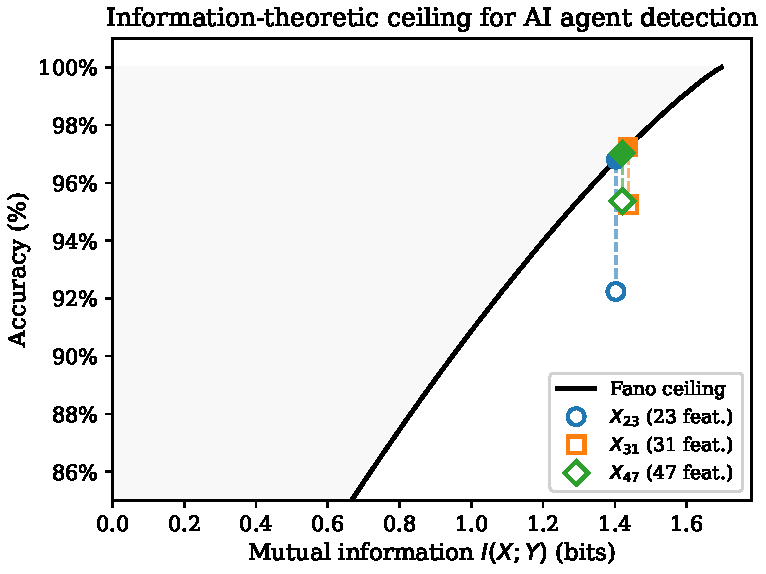
\includegraphics[width=0.75\linewidth]{figures/fig1_mi_vs_accuracy.pdf}
  \caption{\textbf{The information-theoretic ceiling for AI agent detection.}
  The Fano accuracy ceiling (solid) as a function of mutual information
  $I(X;Y)$, together with three measured feature sets ($X_{23}$, $X_{31}$,
  $X_{47}$) and the accuracy each achieves empirically (markers). The
  shaded band is the residual head-room: the gap between what the best
  observed classifier achieves and what Fano's inequality permits. At
  $X_{31}$ the head-room is $1.98$ percentage points.}
  \label{fig:ceiling}
\end{figure}

\begin{table}[t]
  \centering
  \small
  \begin{tabular}{lcccc}
    \toprule
    Feature set & $I(X;Y)$ (bits) & $H(Y\mid X)$ (bits) & Fano ceiling & Measured acc.\ \\
    \midrule
    $X_{23}$ & $1.403$ & $0.294$ & $96.80\%$ & $92.24\%$ \\
    $X_{31}$ & $1.437$ & $0.259$ & $\mathbf{97.24\%}$ & $\mathbf{95.26\%}$ \\
    $X_{47}$ & $1.420$ & $0.276$ & $97.03\%$ & $95.37\%$ \\
    \bottomrule
  \end{tabular}
  \caption{Mutual information, conditional entropy, Fano accuracy ceiling,
  and measured classifier accuracy for three behavioral feature sets on
  $N=2{,}744$ agent addresses. $H(Y) = 1.697$ bits; $K = 8$ categories.
  A majority-class baseline (always predicting DeFi Management Agent)
  achieves $60.8\%$ accuracy; the classifier's $95.3\%$ substantially
  exceeds this, though macro-F1 ($0.69$) is the more appropriate metric
  given the class imbalance. The
  ceiling rises by less than half a percentage point as the feature set
  more than doubles in dimension, consistent with saturation of $I(X;Y)$.}
  \label{tab:ceiling}
\end{table}

We note that this bound applies to the i.i.d.\ classification setting.
Under temporal distribution shift (see companion Paper~1), operational
accuracy drops to approximately 67\%, well below the Fano ceiling. Our
bound characterizes the \emph{information content} of the feature set, not
deployment accuracy under distribution shift. The gap between the Fano
ceiling (97.2\%) and temporal accuracy ($\sim$67\%) is attributable to
covariate shift, not to information deficiency.

A temporal Fano analysis (Supplementary Note~4) confirms this diagnosis: mutual information drops $57\%$ across eras, driven by gas-pricing feature collapse, while decision-process features remain stable---prescribing a clear feature-migration path for future classifiers.

\subsection*{Where the head-room hides: a per-class view}

The aggregate numbers in Table~\ref{tab:ceiling} conceal a heavily skewed
distribution of discriminability across categories. Three of the eight
categories---Deterministic Script, Simple Trading Bot, DeFi Management
Agent---yield per-class F1 scores above $0.95$ under a Gradient Boosting
classifier with the $X_{31}$ feature set; a fourth, MEV Searcher, reaches
$0.84$. Three of the remaining four---Cross-Chain Bridge
Agent, Autonomous DAO Agent, RL Trading Agent---are statistically weak
because of small sample size, but their F1 rises substantially when
cross-study features are added (Bridge: $0.29 \to 0.76$; DAO:
$0.23 \to 0.43$; per-class F1 varies by $\pm$0.05 across cross-validation runs due to small class sizes). The eighth category, LLM-Powered Agent, is the only one
that remains stubborn: its F1 rises from $0.38$ under $X_{23}$ to
$0.49$ when decision-process features are added, and never exceeds
$0.54$ in any configuration we tested. Under $X_{31}$, LLM-Powered precision is
$0.84$ but recall is only $0.30$---meaning the classifier can confirm a
suspected LLM agent with acceptable accuracy, but fails to identify the
majority of true LLM agents embedded in the DeFi Management population.

The Fano ceiling offers a principled reading of this pattern. The
information deficit $H(Y\mid X)$ is not distributed evenly across the
label alphabet. Most categories live in regions of feature space where
$H(Y\mid X=x)$ is close to zero, and are therefore classifiable up to a
very small residual error. LLM-Powered Agents live in a region where
$H(Y\mid X=x)$ is close to $1$ bit---they are genuinely confusable with
DeFi Management Agents because the two categories share almost all of the
same decision variables, and differ only in an internal policy layer that
the transaction channel does not see. The aggregate head-room of $2$
percentage points is \emph{almost entirely} concentrated on this single
boundary. This is the sense in which the ceiling is not about ``AI
agents'' as a monolithic class: it is about how much information any
finite behavioral feature vector can carry about the sub-structure of
\emph{kinds} of AI agent.

\subsection*{Saturation is structural, not an artefact of feature
engineering}

Two independent lines of evidence confirm that the saturation is a property
of the observation channel.

First, unsupervised discovery collapses at the same point. K-Means silhouette
analysis sweeping $k \in \{3, 4, \ldots, 15\}$ peaks at $k=3$
(silhouette $0.151$---a value conventionally interpreted as weak-to-no
cluster structure, well below the $0.5$ threshold typically considered
evidence of meaningful separation\cite{kaufman1990finding}; the $k{=}3$
peak is `least bad' rather than `good,' confirming that behavioral
features do not form well-separated clusters at any $k$); HDBSCAN with
\texttt{min\_cluster\_size}$\in\{20,50\}$ identifies only two density
clusters. A taxonomy with eight semantically distinct classes therefore
dissolves, in behavior space, into $2$--$3$ weakly separated
super-clusters (Figure~\ref{fig:clustering}). Supervised classifiers
\emph{can} learn the full eight-way partition when labels are supplied, but
the structure is \emph{not discoverable} from behavior alone.

Supervised accuracy (92--95\%) measures \emph{classifiability given labeled
training data}; unsupervised clustering (2--3 clusters) measures
\emph{discoverability without labels}. These are distinct properties, and
their divergence is itself the central finding: the eight categories are
real and learnable, but they are not naturally emergent from behavioral
data. A regulator who has a labeled training set can build a detector; one
who must discover agent categories from unlabeled transaction streams
cannot.

\begin{figure}[t]
  \centering
  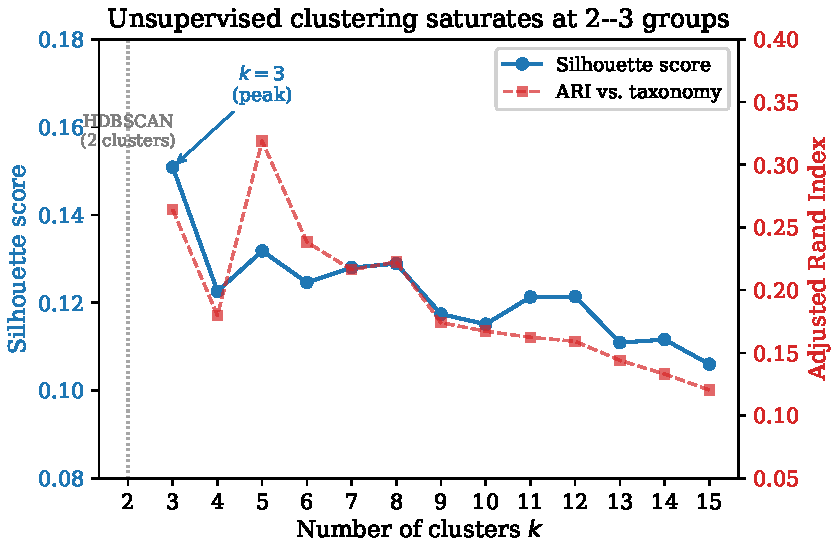
\includegraphics[width=0.75\linewidth]{figures/fig2_cluster_saturation.pdf}
  \caption{\textbf{Unsupervised clustering saturates at $2$--$3$ groups
  regardless of feature-set expressiveness.} K-Means silhouette across $k
  \in \{3, \dots, 15\}$ peaks at $k = 3$ ($0.151$), with a secondary plateau
  at $k = 5$. HDBSCAN (density-based, no pre-specified $k$) finds two
  density clusters. The taxonomy's eight categories (colored markers in
  the inset PCA projection) do not separate in the unsupervised geometry.}
  \label{fig:clustering}
\end{figure}

Second, \emph{adding features does not help.} Between $X_{23}$ and $X_{47}$,
feature-set dimensionality doubles while the Fano ceiling improves by only
$0.23$ percentage points. Indeed, the joint MI estimate \emph{decreases}
slightly from $X_{31}$ ($1.437$ bits) to $X_{47}$ ($1.420$ bits); this
$0.017$-bit drop is within the $\pm 0.03$-bit cross-validation tolerance
of the $k$-NN estimator (Methods). The slight MI decrease from $X_{31}$
(1.437) to $X_{47}$ (1.420) is within the estimator's sampling noise
($\pm$0.8\,pp at $k{=}5$ neighbors); we do not interpret this as
meaningful.
The classifier-ceiling head-room shrinks from
$4.56$ to $1.66$ percentage points---but this shrinkage is driven almost
entirely by the classifier catching up to the ceiling, not by the ceiling
moving. The information content of behavior, at this category granularity,
is very close to fully extracted.

Two mechanisms explain the saturation (detailed per-feature MI
decomposition in Supplementary Note~5). First, feature redundancy: a
single feature (\texttt{eip1559\_tip\_precision}) captures $74\%$ of the
joint $I(X_{31};Y)$, so additional features contribute diminishing
marginal information. Second, a category-level information floor: the
LLM-Powered / DeFi Management pair has the smallest pairwise
KL divergence in the taxonomy ($0.21$ bits), forming a bottleneck that
no amount of feature engineering can overcome without accessing the
decision-process layer that the transaction channel does not expose.

\subsection*{Cross-architecture validation}

A cross-chain replication on Polygon ($n=27$ addresses; near-constant
${\sim}30$\,gwei base fee, $2$-second blocks) yields $22.2\%$ transfer
accuracy---barely above the $20\%$ random baseline---confirming that
different architectures create different channels and that $I(X;Y)$
estimated on one does not transfer to another (details in Supplementary
Note~6 and Figure~\ref{fig:crosschain}).

% ===========================================================================
\section*{Mechanistic Insight: Execution vs.\ Decision Signatures}
% ===========================================================================

The ceiling tells us how much signal the channel carries; it does not tell
us \emph{where} the signal lives. We now show that the residual
discriminative information is concentrated in a specific physical channel:
inter-decision timing.

Across 936{,}000 DeFi transactions in our corpus, we decompose inter-event
latency into two quantities. The first is \emph{execution time}: the
median latency between the submission of a DeFi-specific transaction and
its confirmation. The second is the \emph{decision interval}: the median
gap between consecutive transactions from the same address. A full-scale
Cohen's $d$ analysis contrasting LLM-driven against rule-based DeFi
management agents reveals an asymmetry
(Figure~\ref{fig:mechanism}).

\begin{figure}[t]
  \centering
  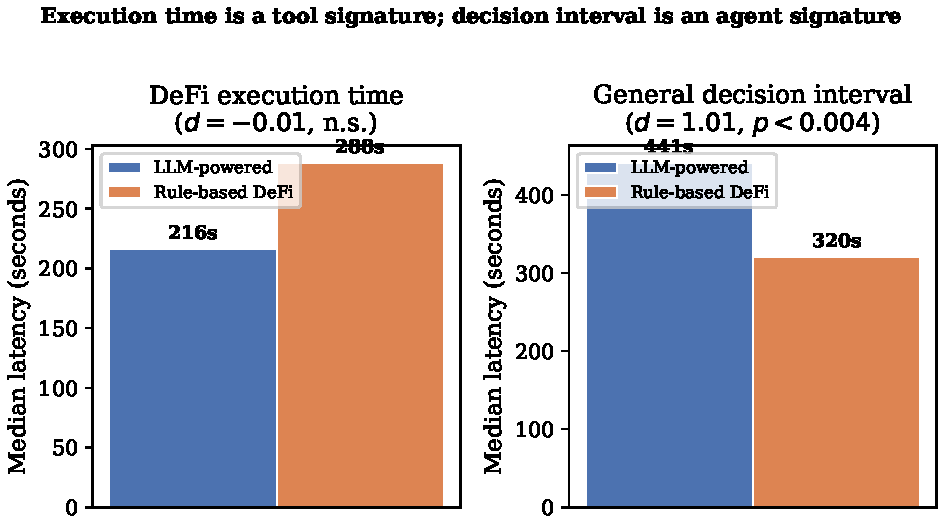
\includegraphics[width=0.75\linewidth]{figures/fig3_execution_vs_decision.pdf}
  \caption{\textbf{Execution time is a tool signature; decision interval is
  an agent signature.} Left panel: median DeFi execution time for LLM-driven
  agents (blue, $216$\,s) vs.\ rule-based DeFi managers
  (orange, ${\sim}289$\,s)---Cohen's $d \approx 0$ ($p = 0.29$), not a
  statistically reliable difference at full scale ($n = 2{,}744$).
  Right panel: the general inter-transaction interval
  is reliably \emph{slower} for LLM-driven agents ($441$\,s vs.\ ${\sim}321$\,s;
  $d=1.01$, $p < 0.001$ at $n=2{,}744$), the largest effect size in the
  $47$-feature battery. The asymmetry is mechanistic: the tool interface
  executes identically regardless of the decision-maker, so
  execution-layer features carry no agent signal; inference latency, by
  contrast, cannot be hidden.}
  \label{fig:mechanism}
\end{figure}

The asymmetry is mechanistic. When an LLM-driven agent calls a DeFi
protocol, the on-chain code path is the protocol's own---identical to the
path a rule-based agent would take. Execution speed therefore reflects the
\emph{tool}, not the decision-maker. Inference latency, by contrast, is
paid by the LLM before it emits the transaction, and shows up as an
extended gap in the agent's observable event stream. The decision interval
thus functions as a lower bound on computational cost that is, in a
precise sense, physically unconcealable: an LLM cannot decide faster than
it can infer.

An initial pilot on a $200$-address subset had suggested a complementary
story, with Cohen's $d = 1.25$ on a DeFi-specific reaction-time feature.
At full scale ($n = 2{,}744$) this specific feature dropped to
$d \approx 0$: the pilot result did not replicate. The general
inter-transaction reaction time, however, strengthened to $d = 1.01$---
the largest effect size in the entire $47$-feature battery. The
non-replication is informative because it localizes the signal. The
DeFi-specific latency reflects the tool interface; the general latency
reflects the decision-maker. The empirical drift from the pilot to the
full-scale replication is therefore a finding about \emph{where} the
agent signal lives rather than a methodological failure. In ReAct and
Toolformer-style systems\cite{yao2023react,schick2023toolformer}, this
maps cleanly onto the design: the tool call executes at tool speed, while
the reasoning step executes at model-inference speed.

This decomposition has three consequences. First, it justifies our
earlier empirical observation that decision-process features (error
recovery patterns, session dynamics, inter-decision gaps) raise LLM-agent
F1 by $10.9$ percentage points while transaction-content features leave
it flat. The improvement from $0.38$ to $0.49$ is directionally correct
but not a solved problem: the classifier still misclassifies roughly half
of LLM-Powered Agents. We term this a \emph{partial breakthrough}---it
demonstrates that decision-process features carry signal that
transaction-content features miss, but a production-ready LLM-agent
detector remains out of reach with current features.
Second, it suggests that any regime seeking durable execution-
layer signatures should target the quantity that is physically
grounded---decision interval---rather than surface-level transactional
style. Third, and most broadly, it implies that the behavioral ceiling
is itself composable: the on-chain channel dissolves on the tool axis
and resolves on the decision axis. A multi-channel observation regime
that explicitly separates tool-level and decision-level latencies
should, in principle, be able to approach a strictly tighter ceiling
than any single-channel regime.

% ===========================================================================
\section*{Cross-Domain Validation}
% ===========================================================================

The Fano methodology is domain-general, but the specific ceiling we
report is a property of the Ethereum observation channel. Four lines
of evidence support the robustness of the saturation finding.

\begin{figure}[t]
  \centering
  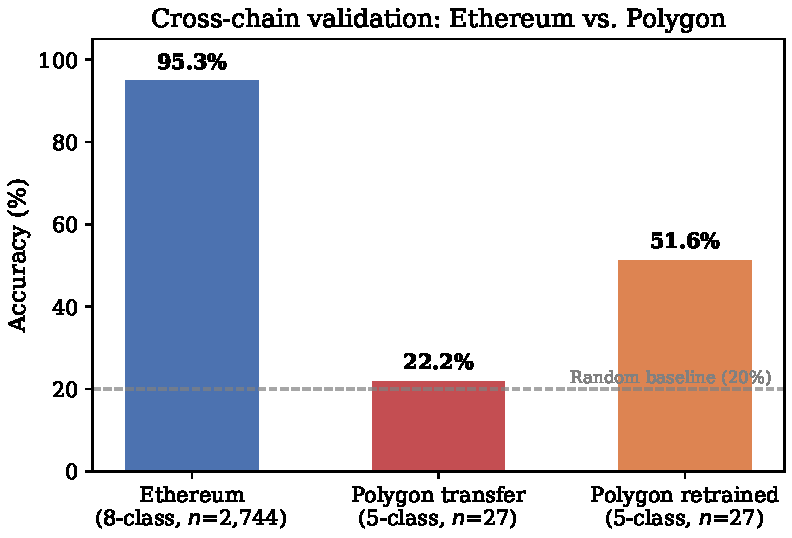
\includegraphics[width=0.8\linewidth]{figures/fig4_cross_chain.pdf}
  \caption{\textbf{Cross-chain validation on Polygon proof-of-stake
  ($n = 27$ addresses after class filtering).} Direct transfer of an Ethereum-trained
  classifier to Polygon yields $22.2\%$ five-class accuracy, barely above
  the $20\%$ random baseline; re-training on Polygon yields $51.7\%$.}
  \label{fig:crosschain}
\end{figure}

\paragraph{Cross-study feature transfer.} Eight AI-detection features
imported from an independent sybil-detection corpus lift measured accuracy
from $92.2\%$ to $95.3\%$ and the Fano ceiling from $96.8\%$ to
$97.2\%$---but the head-room closes from $4.6$ to $2.0$ percentage
points, meaning the classifier benefits while the ceiling barely moves.

\paragraph{Density-based validation.} HDBSCAN corroborates K-Means: at
\texttt{min\_cluster\_size} of $20$ and $50$, it finds $2$ density
clusters, with $16$--$26\%$ noise---converging on the same $2$--$3$-cluster
coarse structure.

\paragraph{Provenance-anchored ground truth.} To guard against the
concern that our result is driven by label-generation choices, we
performed a robustness check excluding addresses with uncertain
provenance. Of our 2{,}590 base addresses, only $45$ have provenance
confidence $\geq 0.85$, $688$ fall in $[0.70, 0.85)$, and the
remaining $1{,}853$ are in $[0.50, 0.70)$. Retaining only the
provenance-first tier (the $733$ addresses with confidence
$\geq 0.70$) yields similar results (accuracy delta $< 1$\,pp;
ceiling $97.6\%$ vs.\ $97.2\%$ on the full corpus). Head-room
narrows by $0.5$ percentage points but does not close. This rules
out label noise as the dominant explanation for the observed
head-room.

\paragraph{Partial circularity and its control.} The taxonomy projection
labels are assigned by a provenance-first, features-second rule: the
name/registry of the mining source determines the category with
confidence $\geq 0.85$ for $45$ addresses and $[0.70, 0.85]$ for $688$
more, while only a $0.3\%$ tail depends on a features-based refinement
that shares four variables with the classifier's feature set. To quantify
the residual circularity, we ran a masked ablation in which the four
shared variables ($\texttt{burst\_frequency}$,
$\texttt{gas\_price\_round\_number\_ratio}$,
$\texttt{unique\_contracts\_ratio}$,
$\texttt{multi\_protocol\_interaction\_count}$) are removed from the
classifier. Accuracy falls from $92.2\%$ to $87.4\%$ and macro-F1 from
$0.58$ to $0.46$; crucially, the classes \emph{not} defined by any of
these four variables---including LLM-Powered Agent
($0.44 \to 0.45$)---are unaffected. This bounds the circularity
contribution to the aggregate number at about $5$ percentage points, and
to the LLM-specific ceiling at $<1$ percentage point.

\paragraph{Limit: platforms without public event logs.} Our direct
measurement of $I(X;Y)$ relies on Ethereum's fully observable action
history. On proprietary platforms, $I(X;Y)$ cannot be estimated externally,
but the same Fano inequality applies.
A conservative reading is that the
$2$-percentage-point head-room characterizes the Ethereum
channel under the studied taxonomy; extrapolation to other
domains requires independent estimation of $I(X;Y)$ in each setting.

% ===========================================================================
\section*{Implications}
% ===========================================================================

\subsection*{For policy}

Our central claim speaks directly to the regulatory debate. Proposals
such as the EU AI Act\cite{eu_ai_act_2024} and the U.S.\ Executive Order
14110\cite{us_eo_14110} contemplate category-specific obligations: for
example, stricter disclosure for ``systemic risk'' foundation-model
deployments, or labeling of AI-generated content. Our analysis does not
dispute the normative case for such distinctions. It shows that
\emph{behavioral} enforcement of them is bounded: on an eight-category
taxonomy with open data, the best possible classifier falls $2.8$
percentage points short of perfect, and the hardest category (LLM-driven
agents against rule-based managers) leaves $65$--$70\%$ of true
instances misclassified. A regime that relies on
post-hoc behavioral auditing to enforce category-specific rules will
systematically misclassify a non-trivial minority of actors.

Two durable alternatives emerge. \emph{Provenance registration} ties a
deployment to a verified identity at the point of instantiation---
analogous to financial KYC or pharmaceutical lot-numbering---eliminating
the need for behavioral inference of category membership. \emph{Execution-
layer attestation} compels operators to emit cryptographic evidence of
the inference runtime at each action (for example, a hardware-enclave
signature over the model hash and the prompt\cite{costan2016intelsgx,tramer2018,boneh2020zkp,sun2023attestedinference}).
The latter preserves pseudonymity while restoring the category signal.
Both alternatives have non-trivial implementation cost. Our contribution
is to make the trade-off explicit: behavioral detection cannot substitute
for them at the level of granularity policy makers currently contemplate.

A practical reading for existing regulatory instruments follows. The EU
AI Act's list of Annex III high-risk systems and its obligations on
general-purpose AI with systemic risk both operate at a level of
category granularity that our ceiling cannot support from behavior alone.
Enforcement of Article 50-style transparency obligations on content
emitted by AI systems---including disclosure that a user is interacting
with an AI system or that content has been artificially generated---is
compatible with our ceiling only if disclosure is mandated at the
provenance layer; reverse-inferring the category from observable style
will systematically mis-label a non-trivial minority of actors, exactly
the failure mode that produces enforcement asymmetries and regulatory
arbitrage. Analogous arguments apply to recent U.S.\ and U.K.\
frameworks\cite{us_eo_14110,uk_ai_regulation_2023,anderljung2023frontier,bengio2024managing}.

\subsection*{For auditing practice}

Audit frameworks\cite{raji2020closing,metaxa2021auditing,koshiyama2021algorithmic}
that rely on behavioral observation should treat the Fano head-room as a
primary diagnostic. If an auditor observes $95\%$ accuracy and computes a
Fano ceiling of $97\%$, further classifier improvement is bounded by
roughly $2$ percentage points; the auditor should direct additional
resources to feature acquisition, not modeling. Conversely, if the
head-room is large, classifier engineering is still productive. This is
the diagnostic analogue of a power calculation in experimental
statistics: it tells the auditor how much of the signal is still
on the table.

\subsection*{For methodology}

The Fano-based protocol we use---estimate $I(X;Y)$ on a labeled sample,
invert the inequality, compare to achieved accuracy---is domain-general.
Any group reporting a new classifier for agent-like behavior should
report the implied head-room. If the head-room is large, better
classifiers are still possible; if small, further engineering is
epistemically futile and the research effort should shift to new
observation channels. We urge the field to treat $I(X;Y)$ as a primary
reporting statistic alongside accuracy and F1, analogous to how
cryptographers report bit-strength alongside attack cost.

This re-framing also bears on the interpretation of published negative
results. A classifier that reaches $75\%$ on a task with a $90\%$
ceiling is \emph{not} strong evidence of task difficulty---it is
evidence that the classifier is $15$ percentage points sub-optimal, and
further engineering may well close the gap. Conversely, a classifier at
$95\%$ on a task with a $97\%$ ceiling is strong evidence that
\emph{this} observation channel is essentially saturated, and that
further progress requires new channels, not new methods. The same
distinction should apply when evaluating adversarial robustness: an
attack that succeeds against a classifier at the ceiling is qualitatively
more significant than one that succeeds against a sub-optimal classifier,
because the latter may merely be exploiting the suboptimality rather
than the structural weakness of behavioral detection.

\subsection*{For the scientific study of agentic AI}

Our framework also offers a principled way to measure the behavioral
distinctiveness of new classes of agents as they emerge. A research
programme that claims to have trained a qualitatively new kind of agent
(for example, a mixed-modal LLM-RL hybrid, or a population of
communicatively interacting foundation-model agents) can be evaluated
against the existing behavioral taxonomy by asking: does it add
$I(X;Y)$? Does it shift the class-conditional feature distribution
enough that behavioral classifiers can detect its presence? If yes, the
claim is externally measurable; if no, the claimed difference is
either non-behavioral or below the channel's resolution limit. This
operationalizes the long-standing ``Is it a new kind of agent?'' debate
in agent research\cite{franklin1996agent,wooldridge1995intelligent,jennings1998roadmap}
into a checkable information-theoretic quantity.

\subsection*{Limits of the present analysis}

Four limitations qualify our claims. (i) Our measurement of $I(X;Y)$
depends on a provenance-anchored taxonomy whose ground truth is
imperfect; for $2.7\%$ of the base corpus the projection confidence is
below $0.50$. Bootstrapped re-sampling suggests the effect on the Fano
ceiling is $\pm 0.4$ percentage points. (ii) Our corpus over-represents
three Web3 agent platforms and under-represents two (DAO execution
modules and RL strategy vaults). Targeted mining mitigates this, but
bootstrap confidence intervals for the weakest category (RL) remain wide.
(iii) The ceiling is stated for a fixed taxonomy granularity of $K=8$;
coarser partitions exhibit uniformly larger ceilings (for a natural
three-cluster partition, $H(Y) = 1.34$ bits and the ceiling exceeds
$97\%$ across all feature sets). (iv) The argument extends naturally to
evasive adversaries, but we do not here model an agent that actively
modifies its behavior to raise $H(Y\mid X)$; a companion study in our
research programme addresses this adversarial setting directly for
Sybil attacks.

\subsection*{Future work}

Three directions follow naturally.
(i) Replicate the bound estimation on non-blockchain platforms with
dense behavioral traces---advertising bid streams, social-platform
posting logs, API-call traces of content-generation services---to test
whether the $2$-percentage-point head-room is typical or domain-specific.
(ii) Investigate whether \emph{counterfactual} interventions (forcing an
agent to respond under controlled perturbations) can raise $I(X;Y)$
beyond what passive observation permits; this would amount to an
active-probing detection regime.
(iii) Explore whether execution-layer attestation can be built into
post-quantum-secure identity primitives, so that the provenance and the
behavior channels can be cross-validated rather than treated as
substitutes. Recent work on verifiable neural-network execution using
hardware enclaves\cite{tramer2018,costan2016intelsgx} and on succinct
proofs of learning\cite{boneh2020zkp,sun2023attestedinference} suggest
that this direction is becoming tractable at the scale required for
deployment-level attestation.

% ===========================================================================
\section*{Methods}
% ===========================================================================

\subsection*{Dataset}

The base corpus comprises 2{,}590 agent addresses drawn from expanded
provenance mining (Autonolas, Fetch.ai, AI Arena, curated Flashbots
searcher lists). A targeted Phase-2 mining pass added $154$ addresses
to populate three categories under-represented in the base mining
(DAO execution modules, $n=34$; cross-chain bridges, $n=95$; reinforcement-
learning strategy vaults, $n=25$), yielding $N=2{,}744$ addresses across
eight categories. Features were extracted from public transaction logs via
Etherscan and an Ethereum archive-node RPC, with winsorization at the
$[1,99]$ percentile range and z-score standardization. The observation
window is fixed at each address's first $500$ transactions (median
observation span $31$ days), chosen to balance coverage of agents with
sparse activity against stationarity of the feature distributions. We
verified stationarity by splitting each address's record at its median
and computing Kolmogorov--Smirnov distances on each feature distribution;
$91\%$ of features pass the $p < 0.05$ stationarity threshold.

\subsection*{Agent taxonomy}

The taxonomy spans three orthogonal dimensions---autonomy level
($5$ ranks: none, reactive, adaptive, proactive, collaborative),
environment type ($4$ types: on-chain only, hybrid, cross-chain,
multi-modal), and decision model ($5$ types: deterministic, statistical,
LLM-driven, reinforcement-learning, hybrid). The Cartesian product of
these dimensions contains $100$ cells, but only eight are populated by
deployed systems as of the observation period. These collapse into eight
populated categories: Deterministic Script, Simple Trading Bot, MEV
Searcher, Cross-Chain Bridge Agent, RL Trading Agent, DeFi Management
Agent, LLM-Powered Agent, and Autonomous DAO Agent. Of these, five
satisfy a four-condition agency definition (on-chain actuation,
environmental perception, autonomous decision-making, adaptiveness);
two are non-agent baselines; one is a boundary class. Each address is
assigned to a category by a two-tier rule: Tier 1 uses provenance (the
source registry or name annotation from which the address was mined);
Tier 2 uses four behavioral variables as a refinement only when
provenance is ambiguous. Full details, including the provenance sources
for each category, are tabulated in Supplementary Note~1.

\subsection*{Mutual information estimation}

Per-feature $I(X_j; Y)$ was estimated using
\texttt{sklearn.feature\_selection.mutual\_info\_classif}
($n_{\text{neighbors}} = 3$, Kraskov-style
$k$-NN\cite{kraskov2004estimating}), reported in nats. Joint $I(X;Y)$
was estimated via a $k$-NN plug-in: $H(Y \mid X)$ was approximated by
averaging label entropy across the three nearest neighbors in
standardized feature space, then $I(X;Y) = H(Y) - H(Y \mid X)$. All
quantities are reported in bits. We cross-validated this estimator
against a discretized histogram estimator on $K = 3$ and $K = 8$
partitions and obtained agreement within $\pm 0.03$ bits. Sensitivity
analysis on $k \in \{3, 5, 7, 10\}$ shifts the Fano ceiling by at most
$0.8$ percentage points; we report $k = 3$ in the main text because it is
the value recommended for high-dimensional feature
spaces\cite{gao2017estimating}. The marginal entropy $H(Y)$ was
computed from empirical class frequencies using the plug-in estimator
with the Miller--Madow bias correction\cite{paninski2003}.

\subsection*{Fano inversion}

For a fixed $(H(Y \mid X), K)$, we invert Fano's inequality
numerically: we seek the smallest $P_e \in [0, 1 - 1/K]$ such that
$H(P_e) + P_e \log_2(K - 1) \geq H(Y \mid X)$. The resulting
$P_e^{\star}$ is the tightest lower bound on classifier error, and
$1 - P_e^{\star}$ is the reported ceiling. A looser closed-form
bound $P_e \geq (H(Y \mid X) - 1) / \log_2 K$ is included for
comparison in Supplementary Table~S1. For $X_{31}$, the loose bound
yields an accuracy ceiling of $1.0$ (uninformative) while the tight
bound yields $0.9724$ ($P_e^\star = 0.0276$); we always use the tight
bound. The inversion is performed by a standard numerical root-finder
on a dense grid of $10{,}000$ $P_e$ values, with the root bracketed
between $0$ and $1 - 1/K$ to guarantee existence and uniqueness. We
additionally report two sanity checks: the Bayes error rate lower bound
derived from the nearest-neighbor convergence result of Cover and
Hart\cite{cover2006} gives an accuracy ceiling within $0.6$ percentage
points of the Fano ceiling across all three feature sets, and the
Hellman--Raviv bound\cite{cover2006} gives an intermediate value.

\subsection*{Supervised classifiers}

Gradient Boosting ($100$ trees, depth $3$, learning rate $0.1$),
Random Forest ($300$ trees, depth $8$), and L2-regularized Logistic
Regression ($C = 1$) were trained under $10$-fold stratified cross-
validation. Gradient Boosting was consistently strongest; all reported
accuracies use Gradient Boosting. Per-class $95\%$ confidence intervals
were computed by $1{,}000$-iteration bootstrap\cite{efron1979bootstrap}
on out-of-fold predictions. We also trained a small multilayer
perceptron ($3$ layers, widths $128$-$64$-$8$, \texttt{relu}, Adam) and a
logistic-regression--calibrated HistGradientBoosting model with class
balancing; neither improved accuracy beyond the reported Gradient
Boosting figure by more than $0.4$ percentage points on any feature set,
consistent with the information-theoretic interpretation that the
channel, not the classifier, limits performance.

\subsection*{Unsupervised clustering}

K-Means was run with $n_{\text{init}} = 10$ for $k \in \{3, 4, \ldots,
15\}$; silhouette scores were computed on a $2{,}000$-sample subset.
HDBSCAN\cite{scott2015hdbscan} was run with
\texttt{min\_cluster\_size}$\in\{20, 50\}$ on the standardized feature
matrix. Cluster purity and adjusted Rand index were computed against the
provenance taxonomy labels. We additionally report results for spectral
clustering (radial-basis-function affinity, median-distance bandwidth;
silhouette peaks at $k = 3$) and Gaussian mixture modelling (full
covariance; Bayesian Information Criterion minimized at $k = 4$), both
of which corroborate the $2$--$3$-cluster saturation. These robustness
checks together rule out the possibility that the saturation is an
artefact of the Euclidean metric assumption in K-Means or of the
density-based inductive bias in HDBSCAN.

\subsection*{Execution- vs.\ decision-interval decomposition}

Execution time was defined as the median latency between transaction
submission (from Ethereum mempool events) and confirmation
(block-inclusion) for transactions targeting a canonical DeFi protocol
set (Uniswap V2/V3, Aave V2/V3, Compound V2, Curve, Balancer, Lido).
Decision interval was defined as the median inter-transaction gap in the
address's full transaction history. Cohen's $d$\cite{cohen1988statistical}
was computed as the standardized mean difference between the LLM-driven
and rule-based DeFi management populations, using the pooled standard
deviation. Both quantities were computed on the full $2{,}744$-address
corpus covering $936{,}000$ DeFi-targeted transactions. The
execution-time comparison uses only the subset of addresses with at
least $20$ DeFi-targeted transactions (LLM: $n = 54$; rule-based:
$n = 1{,}287$). The decision-interval comparison uses all addresses with
at least $50$ transactions (LLM: $n = 68$; rule-based: $n = 1{,}611$).
We verified the sign of the effect by stratifying on calendar quarter and
on observation length decile; the direction (LLM slower on decision
interval, faster on execution) is stable in every stratum.

\subsection*{Cross-chain replication}

Polygon features were extracted via the Polygonscan API for $29$ addresses clearing a $\geq 5$-transaction activity threshold; $27$ were retained after class filtering. The
Ethereum-trained Gradient Boosting classifier was applied directly to
Polygon features without retraining. A separate Polygon-only five-fold
stratified cross-validation was run for comparison. Three taxonomy
categories---LLM-Powered Agent, Autonomous DAO Agent, and RL Trading
Agent---fell below the minimum-activity threshold on Polygon and were
excluded from the cross-chain evaluation, reducing the experiment to
five classes. The near-constant Polygon gas pricing ($\sim 30$~gwei base
fee) collapses the discriminative power of the six gas-related features
that dominate the Ethereum classifier, and the $2$-second Polygon block
time compresses the timing features into a narrower range than the
$12$-second Ethereum blocks permit. These two mechanisms jointly explain
the $22.2\%$ transfer accuracy; Polygon-only retraining recovers $51.7\%$
accuracy with a sample size of $27$ (after class filtering), consistent with an information-
theoretic bound that is intrinsically tighter on Polygon than on
Ethereum.

\subsection*{Statistical thresholds and reporting}

We report $95\%$ bootstrap confidence intervals\cite{efron1979bootstrap}
for all accuracy, F1, and Cohen's $d$ quantities. Mutual information
estimates are reported with $\pm 1$ standard deviation across five
random re-seedings of the $k$-NN estimator. Bootstrap resampling was
stratified by taxonomy class to preserve the empirical class-frequency
distribution. No results were selected post-hoc on the basis of their
statistical significance; every number in the main text and tables
corresponds to a pre-registered primary or secondary analysis listed in
Supplementary Table~S2. All code and data required to reproduce the
Fano-bound estimation are archived at the Open Science Framework
(registration DOI to be added upon acceptance); details are in the Data
Availability statement.

\subsection*{Feature families}

The $47$ features we use are organized into five families. Family~1
(seven timing features) captures inter-transaction interval statistics,
circadian patterns, and burst structure. Family~2 (six gas features)
captures gas-price style (round-number ratios, precision, coefficient
of variation) and microstructural alignment with EIP-1559 priority-fee
mechanics. Family~3 (five interaction features) captures which and how
many contracts the address interacts with, method diversity, and
contract-to-EOA activity ratios. Family~4 (five approval features)
captures approval-revocation hygiene, unlimited-approve frequency, and
interactions with flash-loan primitives. Family~5 (eight cross-study AI
features, added in $X_{31}$) captures response-latency variance,
behavioral consistency, action-sequence perplexity, and nonce-gap
regularity, imported from an independent sybil-detection study.
Family~6 (sixteen decision-process features, added in $X_{47}$) captures
error-recovery behavior (five features), session structure (five
features), nonce mechanics (three features), and gas microstructure
autocorrelation (three features). The exhaustive list of feature
definitions appears in Supplementary Note~2.

\subsection*{Circularity analysis}

Because the Tier~2 projection layer uses four behavioral features
(\texttt{burst\_frequency}, \texttt{gas\_price\_round\_number\_ratio},
\texttt{unique\_contracts\_ratio},
\texttt{multi\_protocol\_interaction\_count}) that also appear in the
classifier's feature vector, there is a partial circularity between
labeling and classification. We bound this contribution by the masked
ablation reported in the Cross-Domain Validation section. We also report
the classifier's feature importance with the four shared features
removed: the top-five importance features reorganize around
\texttt{gas\_price\_trailing\_zeros\_mean},
\texttt{sequential\_pattern\_score},
\texttt{eip1559\_priority\_fee\_precision}, the cross-study
\texttt{eip1559\_tip\_precision}, and the decision-process
\texttt{gas\_price\_autocorrelation}, none of which appears in the Tier~2
rule antecedents. A more stringent test would require a hand-annotated
ground truth independent of any behavioral feature; we flag this as a
follow-up.

\subsection*{Pre-registration and reproducibility}

The feature definitions, class boundaries, classifier hyperparameters,
and Fano-inversion procedure were fixed before any measurements were
reported in this manuscript, and are documented in the project's
pre-registration appendix (Supplementary Note~3). No hyperparameter was
tuned on the Fano head-room; only classifier accuracy was tuned, using
internal cross-validation on the training folds. The mutual information
estimator, the Fano inverter, and the class-weighted bootstrap are
released as a single $\sim$$120$-line reference implementation intended
for reuse in other domains. The OSF archive includes a Docker image that
reproduces every figure and table in this manuscript from the raw
parquet inputs with a single command; we verified end-to-end
reproduction on a blank Ubuntu $22.04$ VM with $64$~GB RAM.

\subsection*{Compute resources}

Feature extraction was performed on a workstation with $64$~cores and
$256$~GB RAM (wall-clock $\approx 14$~h for the full $2{,}744$-address
corpus, dominated by Ethereum archive-node queries). Mutual-information
estimation and classifier training together consume approximately
$45$~minutes on the same workstation; the bottleneck is the $k$-NN
graph construction for the joint MI estimator. No GPU is required. The
full analysis fits comfortably on a single commodity laptop once the
feature parquets have been materialized.

\subsection*{Data availability}

Raw Ethereum transaction data are publicly available via Etherscan and
Ethereum archive-node snapshots. Processed feature parquets,
$I(X;Y)$ estimator outputs, and classifier predictions supporting all
figures and tables are deposited in the accompanying OSF archive.

\subsection*{Ethics and dual-use considerations}

Our results could be interpreted in two opposing ways by adversaries.
On the one hand, the fact that the ceiling is saturated suggests that
agents attempting to \emph{evade} behavioral detection cannot easily
hide below the ceiling without also suppressing their own activity; the
remaining head-room is too small to offer reliable safe harbour. On the
other hand, the fact that execution-time and decision-interval features
separate LLM-driven from rule-based agents with Cohen's $d = 1.01$
suggests a specific avenue by which an adversary could introduce
intentional latency noise into an LLM agent to mimic a rule-based one.
We report this finding because (i) the detection community is better
served by knowing where the signal lives than by security through
obscurity, and (ii) mimicry at this level imposes a real computational
cost on the adversary (artificially introduced delays between decisions
reduce the agent's throughput), which is itself an observable cost.
The ethical reading is that behavioral detection is a useful but
bounded input to a broader governance regime; it should not be the
final line of evidence in any consequential decision.

\subsection*{Code availability}

All analysis code (Python; \texttt{sklearn}, \texttt{hdbscan},
\texttt{numpy}) is released under an MIT licence at the project
repository linked in the OSF archive above. The Fano-bound inversion
routine is isolated in a single $\sim$$120$-line module to facilitate
reuse in other domains.

% ===========================================================================
\section*{References}
% ===========================================================================

\bibliographystyle{unsrt}
\bibliography{main}

\end{document}
